\documentclass{article}

\usepackage{graphicx}
\usepackage{amsmath}
\usepackage{amssymb}
\usepackage{bbm}
\usepackage{subcaption}
\usepackage{hyperref}

\title{6.865 Pset 10: Edge Cameras in Julia}
\author{Robin Deits}
\date{\today}

\begin{document}

\maketitle

\section{Introduction}

Just as a pinhole camera creates an image of a scene by blocking all light rays except those passing through a single point, other obstructions in an environment can create partial images of the scene beyond. In particular, a sharp edge can act as a partial pinhole camera in one dimension, casting a shadow which minutely varies based on the illuminated objects on the other side of that edge \cite{bouman_turningcornerscameras2017}. In \cite{bouman_turningcornerscameras2017}, the authors demonstrate a method to turn vertical edges formed by walls and doorways into \emph{edge cameras}, which allow a 1-D reconstruction of an occluded scene. The only input required by the algorithm is a video of the floor near the edge, and the reconstruction can be run over a period of time to build up a time-space image of motion in the occluded scene. 

For my 6.865 final problem set, I have re-implemented the core edge camera algorithm, and used it to demonstrate reconstruction of motion from one camera as well as reconstruction of 2-D motion from a stereo pair of edge cameras. 

\section{Related Work}

There have been a variety of approaches to use naturally occurring elements of an environment to reveal otherwise hidden scenes. In \cite{torralba_accidentalpinholepinspeck2012}, the authors use, variously, a window, an arm, a thrown ball, and an entire human figure as pinhole or pinspeck cameras, extracting images of the world from subtle variations caused by changes in occlusion. The authors of \cite{zhang_sparklevisionseeing2014} use inference to estimate the image mapping created by a random specular surface. From this mapping, they are able to reconstruct an image reflected and scattered by a surface covered in glitter. In \cite{nishino_eyesrelighting2004}, the reflective surface of the human cornea is likewise used to reconstruct the illumination of a scene. Finally, in \cite{fergus_randomlensimaging2006}, the authors infer the transfer function for an uncalibrated, pseudo-random lens in order to reconstruct scenes viewed through the lens. 

A distinction of the particular work in \cite{bouman_turningcornerscameras2017} and reproduced here is that it operates on one-sided edges, rather than pinholes or slits. Where a slit would create a 1-D pinhole image on its own, a corner requires an analysis of the variation in the image as a function of angle with respect to the corner in order to reproduce the hidden scene. 

\section{Algorithm}

The edge camera algorithm is discussed in detail in \cite{bouman_turningcornerscameras2017} but will be summarized here as well. To generate input to the algorithm, we record a video of the ground near a corner while a subject walks back and forth around the corner. Each frame of the video is processed by first subtracting the background image. Since a perfect background image may not be available, we substitute the mean image over the course of the video, which appears to work well in practice. 

\subsection{Homography}

Calibrating the position and orientation of the edge camera consists of identifying a homography to correct for the position of the corner in the image and any projective distortion. The homography is computed by identifying four points forming a square on the ground, with the first points exactly at the imaging edge. A background image with the four points marked is shown in Fig. \ref{fig:background}. Note that precise calibration of the homography is not required: while a calibration target could be used to get exact locations for each of the four points, the authors in \cite{bouman_turningcornerscameras2017} only needed to count square floor tiles to reconstruct a sufficiently accurate homography. 

\begin{figure}[htbp]
	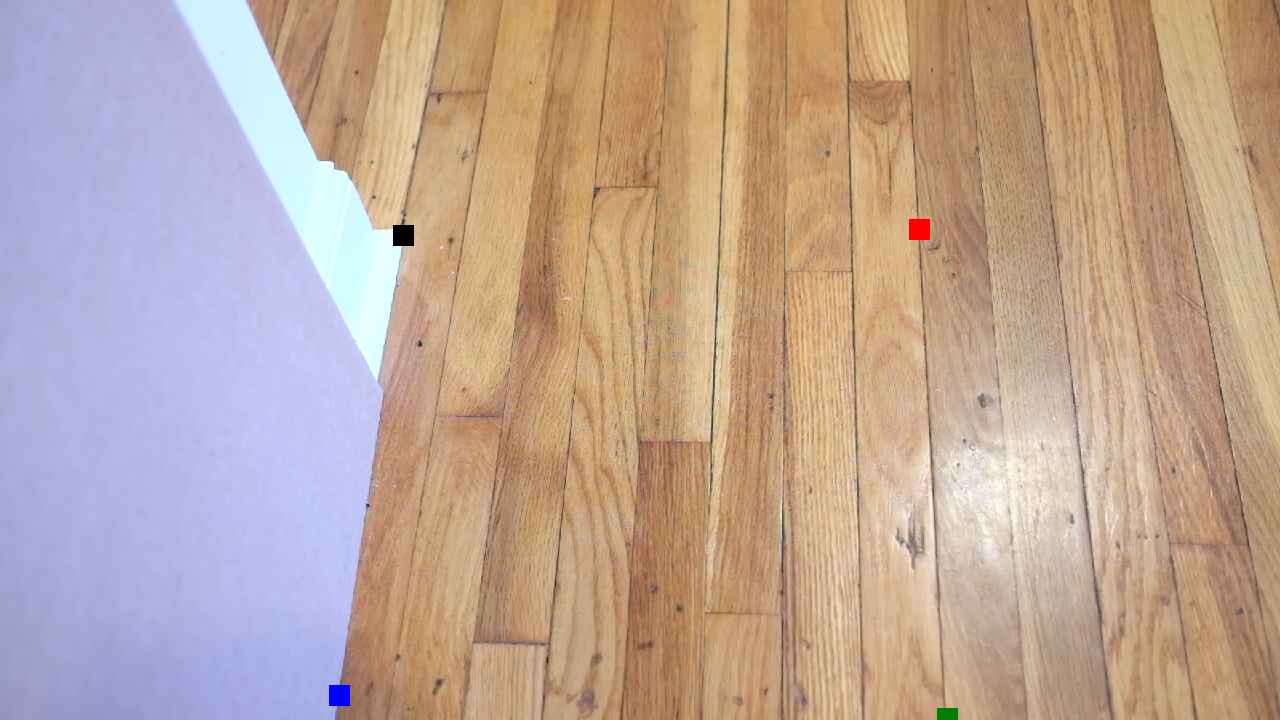
\includegraphics[width=\textwidth]{img/background.png}
	\caption{An example of a background frame with the four homography calibration points indicated. The edge forming our camera is located at the black point, and the subject walks around the corner to the left.}
	\label{fig:background}
\end{figure}

\subsection{Sampling}

Once the homography is computed, a set of regularly spaced samples is chosen within the image. While these samples could be placed in any pattern, calculation of the gradient matrix in Sect. \ref{sec:gain} is simpler if the samples are uniformly distributed in polar coordinates centered on the target edge. Such radially spaced samples can be seen in Fig. \ref{fig:samples}.

\begin{figure}[htbp]
	\begin{subfigure}[t]{0.83\textwidth}
		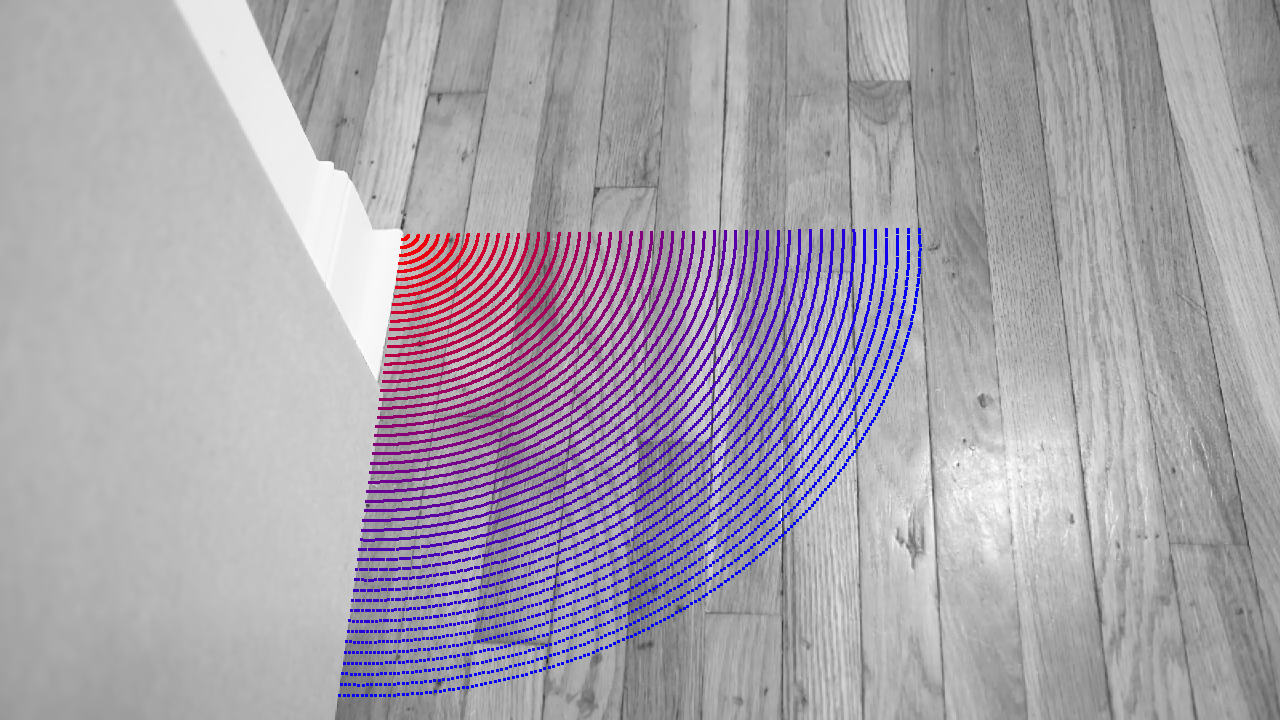
\includegraphics[width=\textwidth]{img/samples.png}
		\caption{Radially spaced sampling locations for extracting edge camera pixels. Color gradient (red to blue) indicates the order in which the pixels are stacked in the $A$ matrix in Sect. \ref{sec:gain}.}
		\label{fig:samples}
	\end{subfigure}
	~
	\begin{subfigure}[t]{0.12\textwidth}
		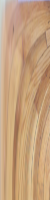
\includegraphics[width=\textwidth]{img/polar_samples.png}
		\caption{Pixels extracted from the sample locations shown in (a).}
	\end{subfigure}
\end{figure}

\subsection{Computing the Gain Matrix}
\label{sec:gain}

The continuous 1-D image of the scene around the corner is discretized into $N$ terms which we will call $\textbf{x}$ (the elements of $\textbf{x}$ are evenly spaced in angle around the camera edge).

Given observations $\textbf{y}$ at each of the sampling locations, we wish to estimate $\textbf{x}$. The observations are related to the unknowns by a linear matrix operator:

\begin{align}
\textbf{y} = L_v + \textbf{A} \textbf{x} + \textbf{w}
\end{align}

where each element of $\textbf{w}$ is drawn from a zero-mean normal distribution with variance $\lambda^2$ and where $L_v$ is a constant offset term. The $\textbf{A}$ matrix is determined by the particular choice of sampling locations: each element $\textbf{A}_{ij}$ is 1 if and only if there is a line of sight from region of the hidden scene corresponding to element $\textbf{x}_j$ to sample $\textbf{y}_i$. 

Full derivation of the MAP likelihood estimation can be found in \cite{bouman_turningcornerscameras2017}, but from a practical perspective the edge camera algorithm amounts to computing a gain matrix $\textbf{K}$ such that

\begin{align}
	\left[ \hat{L}_v \quad \hat{\textbf{x}}^T \right]^T = \textbf{K} \textbf{y}
\end{align}

where 

\begin{align}
	\textbf{K} &= \Sigma \lambda^{-2} \tilde{\textbf{A}}^T\\
	\Sigma &= \left[ \lambda^{-2} \tilde{\textbf{A}}^T \tilde{\textbf{A}} + \begin{bmatrix} 0 & 0 \\ 0 & \frac{\textbf{G}^T \textbf{G}}{\sigma_1^2} + \frac{\mathbbm{1}}{\sigma_2^2} \end{bmatrix} \right]^{-1} \\
	\tilde{\textbf{A}} &= \left[ \mathbbm{1} \quad \textbf{A} \right]
\end{align}

Each video frame produces a new set of samples $\textbf{y}$ from which a new estimate $\textbf{x}$ can be computed. These 1-D estimates can be concatenated to create a 2-D image, with the angularly-spaced elements of $\textbf{x}$ along the first axis and time along the second. Such a space-time reconstruction can be seen in Fig. \ref{fig:trace}. 

\section{Results}

\begin{figure}[htbp]
	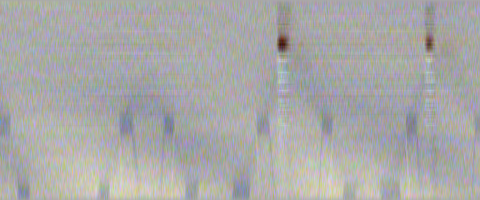
\includegraphics[width=\textwidth]{img/trace.png}
	\caption{Reconstructed space-time image for a hidden scene consisting of one person (the author) walking back and forth three times. This image was generated from the scene shown in Fig. \ref{fig:background} using the approach described in Sect. \ref{sec:gain}. The image was normalized to take values between 0 and 1.}
	\label{fig:trace}
\end{figure}

\begin{figure}[htbp]
	\begin{subfigure}[t]{0.45\textwidth}
		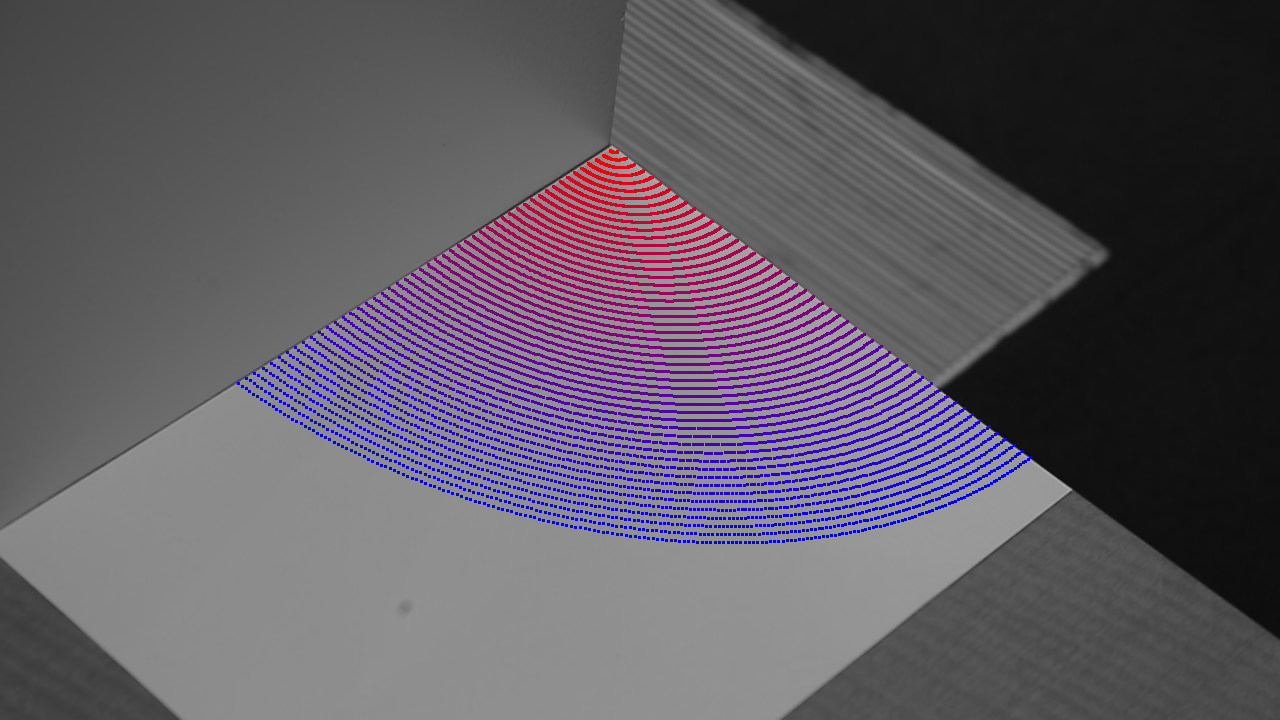
\includegraphics[width=\textwidth]{img/2_people_samples.png}
		\caption{Sampling points.}
	\end{subfigure}
	~
	\begin{subfigure}[t]{0.45\textwidth}
		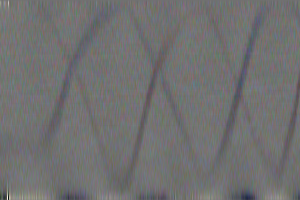
\includegraphics[width=\textwidth]{img/2_people_trace.png}
		\caption{Reconstructed space-time image.}
	\end{subfigure}
	\caption{Edge camera using the video of two subjects from \cite{bouman_turningcornerscameras2017}. Note the blue and red hues of the two lines in (b) caused by the blue and red colors of the hidden subjects' clothing.}
	\label{fig:2_people_samples}
\end{figure}

\begin{figure}[htbp]
    \centering
    \begin{subfigure}[t]{0.45\textwidth}
        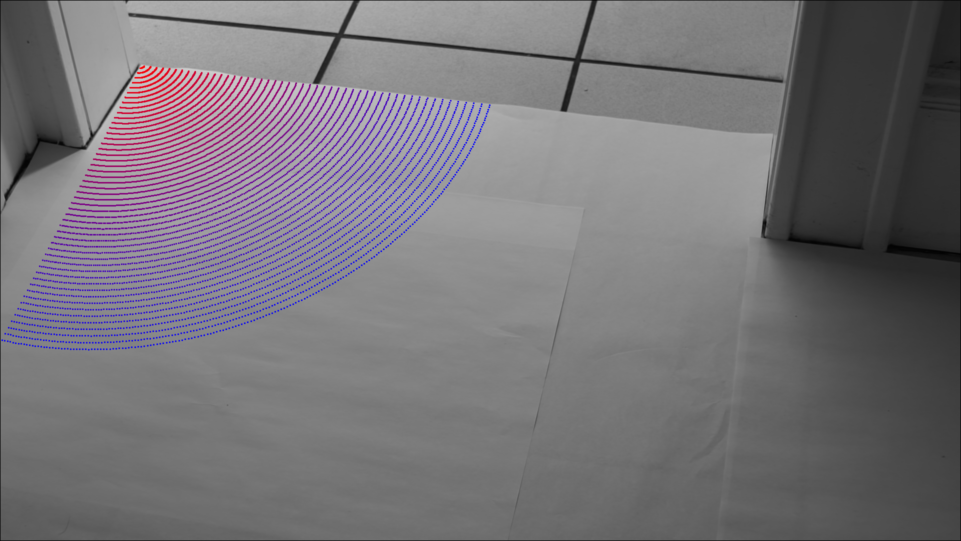
\includegraphics[width=\textwidth]{img/stereo_samples_1.png}
        \caption{Left camera samples.}
    \end{subfigure}
    ~
    \begin{subfigure}[t]{0.45\textwidth}
        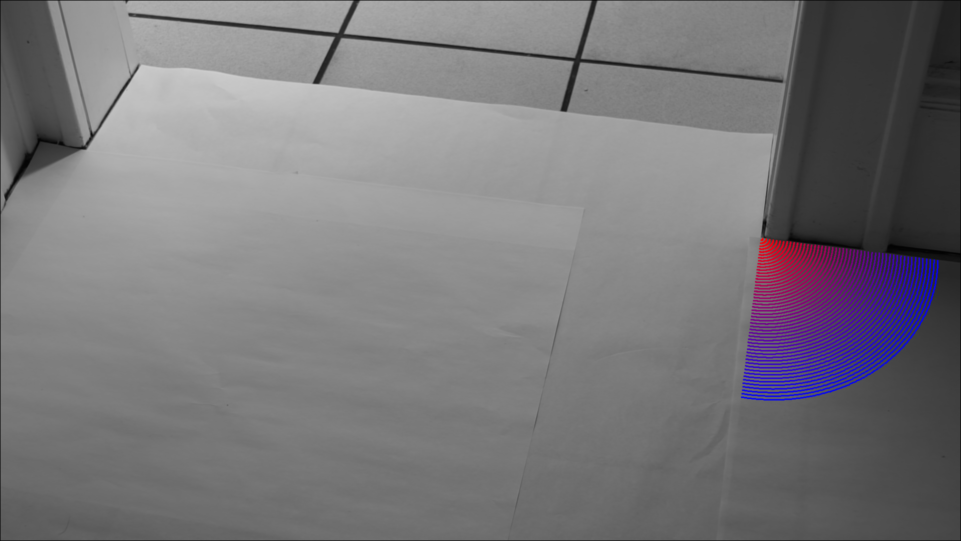
\includegraphics[width=\textwidth]{img/stereo_samples_2.png}
        \caption{Right camera samples.}
    \end{subfigure}

    \begin{subfigure}[t]{0.45\textwidth}
        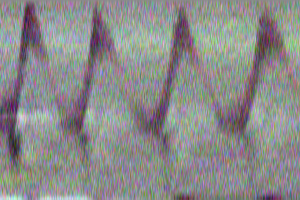
\includegraphics[width=\textwidth]{img/stereo_trace_1.png}
        \caption{Space-time image extracted from the left edge camera.}
        \label{fig:stereo-trace-left}
    \end{subfigure}
    ~
    \begin{subfigure}[t]{0.45\textwidth}
        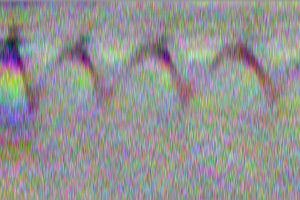
\includegraphics[width=\textwidth]{img/stereo_trace_2.png}
        \caption{Space-time image extracted from the right edge camera.}
        \label{fig:stereo-trace-right}
    \end{subfigure}
    \caption{Using two edge cameras for stereo reconstruction.}
    \label{fig:stereo}
\end{figure}

I ran the edge camera algorithm on three scenes: the indoor scene with two subjects walking (from \cite{bouman_turningcornerscameras2017} and shown in Fig. \ref{fig:2_people_samples}), the indoor stereo scene with two edge cameras and one subject (from \cite{bouman_turningcornerscameras2017} and shown in Fig. \ref{fig:stereo}), and an indoor scene that I recorded myself (shown in Fig. \ref{fig:background}, \ref{fig:samples}, \ref{fig:trace}). Each scene shows a recognizable pattern in the space-time image which corresponds to the motion of the hidden subject. 

With two corner cameras, as in Fig. \ref{fig:stereo}, it is possible to estimate the full 2D position of the hidden subject. Following the derivation in \cite{bouman_turningcornerscameras2017}, I manually traced the apparent path of the subject in Figs. \ref{fig:stereo-trace-left} and \ref{fig:stereo-trace-right} and triangulated the position of the subject from the two angular measurements. The estimated position of the subject is shown in Fig. \ref{fig:2d-path} and is, at least qualitatively, a good fit to the original stereo reconstruction in Fig. 9 of \cite{bouman_turningcornerscameras2017}. 

\begin{figure}[htbp]
	\centering
	\begin{subfigure}[t]{0.45\textwidth}
		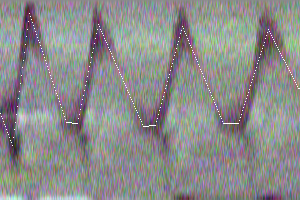
\includegraphics[width=\textwidth]{img/stereo_draw_1.png}
		\caption{Manually traced path in the left camera image.}
	\end{subfigure}
	~
	\begin{subfigure}[t]{0.45\textwidth}
		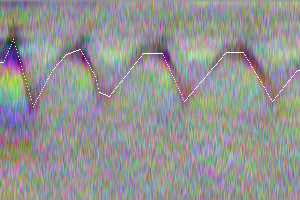
\includegraphics[width=\textwidth]{img/stereo_draw_2.png}
		\caption{Manually traced path in the right camera image.}
	\end{subfigure}

	\begin{subfigure}[t]{0.45\textwidth}
		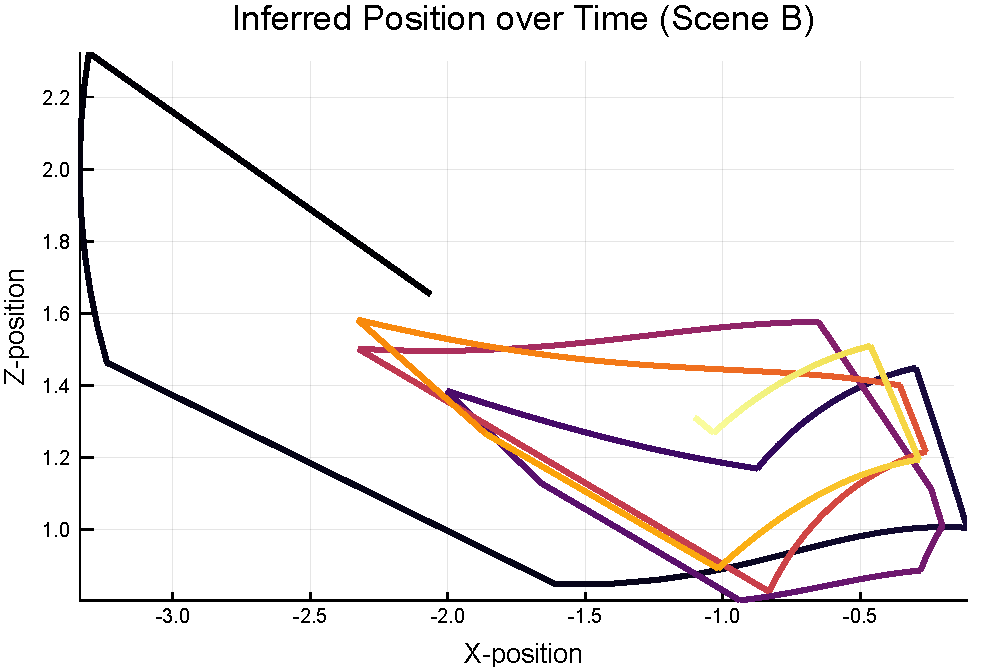
\includegraphics[width=\textwidth]{img/stereo_path.pdf}
		\caption{Two-dimensional position of the hidden subject, estimated by triangulating the two edge camera results in Fig. \ref{fig:stereo}. Compare with the lower right-hand part of Fig. 9 in \cite{bouman_turningcornerscameras2017}.}
		\label{fig:2d-path}
	\end{subfigure}
\end{figure}

\section{Implementation Details}

I chose to implement this project in the Julia programming language \cite{bezanson_juliafreshapproach2017} because its combination of performance, excellent support for mathematical computing, and relatively expressive syntax make it an appealing choice for exploring computational photography. I relied on the JuliaImages \cite{_juliaimages} tools to provide the basic image data structures and handled raw video input using the VideoIO.jl package, a wrapper around ffmpeg. 

Full source code can be found at \href{https://github.com/rdeits/EdgeCameras.jl}{https://github.com/rdeits/EdgeCameras.jl}. Please see the \texttt{Readme.md} file for detailed examples of usage. 

\subsection{Performance}

On an Intel i7 process at 2.5 GHz, my implementation is able to process 1280x720 HD frames at 33 frames per second, which would be sufficient for real-time edge camera processing. From profiling, roughly 60\% of the computation time is spent extracting samples from the image (see Sect. \ref{sec:sampling}), 30\% is spent applying the gain matrix $\textbf{K}$ and 10\% is spent reading frames from the video. There are some clear opportunities for parallelization, as the samples could be collected in parallel, but my implementation is currently single-threaded. 

\subsubsection{Extracting Samples}
\label{sec:sampling}

When extracting the radially-spaced samples $\textbf{y}$ from each video frame, we could simply interpolate within the unmodified frame. However, since the spatial frequency of the sampling points is much lower than the resolution of the image, this would introduce the opportunity for aliasing, which could harm our reconstruction. Instead, we blur each frame with a Gaussian kernel (a standard deviation of 3 to 5 pixels works well in practice) before extracting the samples. Unfortunately, this gives two problems: 

\begin{enumerate}
	\item Blurring the entire HD image is too slow.
	\item Even after blurring, the radially-spaced samples are not at integer pixel coordinates, so we would still need to interpolate.
\end{enumerate}

Rather than blurring the entire image and interpolating, I instead chose to essentially \emph{inline} the blur into the sampling process. 
That is, each time a sample pixel is accessed, I compute its value by applying a Gaussian kernel to the pixels around the sample point. 
However, applying a Gaussian blur at non-integer pixel coordinates requires computing the weights of the Gaussian kernel on-line, which requires one exponential call for each point in the kernel. 
This turned out to be so expensive that calls to the exponential function dominated the entire runtime of my algorithm. 
To solve the problem, I pre-computed Gaussian weights at several non-integer coordinates and then interpolated linearly between them at run-time. 
With just three interpolation points, I was able to match the true Gaussian weights to within a margin of 0.02 while substantially improving performance. 
With Gaussian weights computed on-line, extracting a single pixel blurred with a 13x13 kernel required 2.6\,$\mu$s. Computing the weights by linear interpolation reduced that time to just 600\,ns and approximately doubled the total framerate of my implementation. 

\subsection{Estimating Image Noise}

One aspect of the edge camera algorithm that I have not yet implemented is estimation of the image noise parameter $\lambda$. The authors of \cite{bouman_turningcornerscameras2017} recommend using the median of the variance of the per-pixel noise, but I found that a default value of 1.6 worked well enough in practice. 

\section{Conclusion}

Implementing edge cameras in Julia was relatively straightforward, and I was surprised at how easily the technique could be applied to a new scene without any modification. Despite the interpolation scheme, the sampling of the blurred image is still the major performance bottleneck and will have to be addressed in order to hit framerates better than 30\,Hz. Better noise estimation (the parameters $\lambda$, $\sigma_1$, and $\sigma_2$) may also help produce cleaner results. Finally, automating the manual tracing of the subject's location in the stereo demo would allow for on-line estimation of the subject's position from live video.


\bibliographystyle{plain}
\bibliography{edgecams}

\end{document}
